%% LyX 2.1.3 created this file.  For more info, see http://www.lyx.org/.
%% Do not edit unless you really know what you are doing.
\documentclass[english]{article}
\usepackage{ccfonts}
\usepackage[T1]{fontenc}
\usepackage[latin9]{inputenc}
\usepackage{geometry}
\geometry{verbose,tmargin=3cm,bmargin=3cm,lmargin=3cm,rmargin=3cm,headheight=3cm,headsep=3cm,footskip=3cm}
\usepackage{url}
\usepackage{amsmath}
\usepackage{graphicx}
\usepackage{setspace}
\onehalfspacing

\makeatletter

%%%%%%%%%%%%%%%%%%%%%%%%%%%%%% LyX specific LaTeX commands.
%% A simple dot to overcome graphicx limitations
\newcommand{\lyxdot}{.}


%%%%%%%%%%%%%%%%%%%%%%%%%%%%%% User specified LaTeX commands.
\usepackage{listings}
\usepackage{xcolor}

\makeatother

\usepackage{babel}
\begin{document}

\title{Lorenz Attractors}


\author{Atul Singh Arora}


\date{March-April 2015}

\maketitle

\section{Introduction}

The Lorenz attractor is the consequence of a set of 3 ordinary differential
equations, which for a given range of parameters, results in chaotic
solutions. This is of particular interest because the resultant solutions,
when plotted in 3 dimensional space, move in a very contrained part
of the space, intuitively suggesting that its dimension must be between
1 and 3. What is further fascinating is that even though the solution
is chaotic, it is possible to synchronize two lorenz attractors, which
is to say that while the motion of neither can be modelled (chaotic),
yet both perform the same chaotic motion. In this paper, I show numerically
that the dimension of the `Lorenz attractor' is $\sim2$ and demonstrate
that it is indeed possible to synchronize two lorenz attractors. Further,
a peculiar observation was made; the distance between the two solutions
(a measure of synchrony), although appeared to drop exponentially
initially, in accordance with the theory, there seemed to be a periodic
increase and decrease which I haven't been able to account for theoretically.


\section{Lorenz Attractor, equations}

The lorenz equations are given as

\[
\begin{aligned}\dot{x} & =\sigma(y-x)\\
\dot{y} & =rx-y-xz\\
\dot{z} & =xy-bz
\end{aligned}
\]
where $\sigma,r,b>0$ are parameters. These were designed to model
convection flows in the atmosphere. One can show various interesting
properties of the attractor, including the fact that volumes in phase
space contract under the flow, which results in elimination of existence
of sources/repellers. For $r<1$, it can be shown that the origin
is globally stable. One can further show that, given 

\[
r_{H}\equiv\frac{\sigma(\sigma+b+3)}{\sigma-b-1}
\]
for 
\[
1<r<r_{H}
\]
there exist two more stable fixed points, $C^{+}$ and $C^{-}$. For
$r>r_{H}$ is where there's chaos, where chaos maybe defined as ``aperiodic
long-term behaviour in a deterministic system that exhibits sensitive
dependence on initial conditions''.


\section{Syncing two Lorenz attractors}

Upon appropriate scaling ($u=x/10,v=y/10,w=z/20$), I can define the
same lorenz equations as

\[
\begin{aligned}\dot{u} & =\sigma(v-u)\\
\dot{v} & =ru-v-20uw\\
\dot{w} & =5uv-bw
\end{aligned}
\]
I can couple another lorenz attractor as

\[
\begin{aligned}\dot{u}_{r} & =\sigma(v_{r}-u)\\
\dot{v}_{r} & =ru-v-20uw_{r}\\
\dot{w_{r}} & =5uv_{r}-bw_{r}
\end{aligned}
\]
where note that the coupling is done by replacing $u_{r}$ with $u$.
The claim is that regardless of the initial conditions, both attractors
synchronize nearly perfectly, exponentially fast. This is particularly
interesting because even though we're feeding in the $u$ variable,
the other attractor is able to generate $v$ and $w$ to be in perfect
sync.

Quantitatively, the claim is that if I define
\[
\begin{aligned}\mathbf{x} & =(u,v,w)\\
\mathbf{y} & =(u_{r},v_{r},w_{r})\\
\mathbf{d} & =\mathbf{x}-\mathbf{y}
\end{aligned}
\]
then $d\to0$ as $t\to\infty$. The proof is as follows.
\[
\begin{aligned}\dot{d}_{1} & =\sigma(d_{2}-d_{1})\\
\dot{d}_{2} & =-d_{2}-20ud_{3}\\
\dot{d}{}_{3} & =5ud_{2}-bd_{3}
\end{aligned}
\]
We now construct the following by multiplying the second equation
with $d_{2}$ and the third by $4d_{3}$ and then adding. We have
\[
\begin{aligned}d_{2}\dot{d}_{2}+4d_{3}\dot{d}_{3} & =-d_{2}^{2}-20ud_{2}d_{3}+20ud_{2}d_{3}-4bd_{3}^{2}\\
 & =-d_{2}^{2}-4bd_{3}^{2}
\end{aligned}
\]
where we have managed to remove the $u$ term which was known to be
chaotic. Note also that the left hand side is essentially 
\[
\frac{1}{2}\frac{d}{dt}\left(d_{2}^{2}+4d_{3}^{2}\right)
\]
Next we define the function 
\[
E(\mathbf{d},t)=\frac{1}{2}\frac{d}{dt}\left(\frac{1}{\sigma}d_{1}^{2}+d_{2}^{2}+4d_{3}^{2}\right)
\]
Note now that for $\sigma>0$, $E>0$ for all $t$. If I can show
that $\dot{E}<0$, then that must mean that eventually, $d\to0$.
I have already evaluated two terms in the sum. Lets evaluate the first
term. 
\[
\begin{aligned}\dot{E} & =\left[\frac{1}{\sigma}d_{1}\dot{d}{}_{1}\right]+-d_{2}^{2}-4bd_{3}^{2}\\
 & =-\left[d_{1}^{2}-d_{1}d_{2}\right]-d_{2}^{2}-4bd_{3}^{2}
\end{aligned}
\]
Completing square (for the bracketed term)

\[
\begin{aligned}\dot{E} & =-\left[d_{1}^{2}-d_{1}d_{2}\right]-d_{2}^{2}-4bd_{3}^{2}\\
 & =-\left[d_{1}^{2}-\frac{1}{2}d_{2}\right]^{2}+\left(\frac{1}{2}d_{2}\right)^{2}-d_{2}^{2}-4bd_{3}^{2}\\
 & =-\left[d_{1}^{2}-\frac{1}{2}d_{2}\right]^{2}-\frac{3}{4}d_{2}^{2}-4bd_{3}^{2}
\end{aligned}
\]
So for $b>0$, we know that $\dot{E}\le0$ with equality only if $\mathbf{d}=\mathbf{0}$.
It thus proves that $\mathbf{d}=\mathbf{0}$ is globally stable.


\section{Correlation Dimension}

This is to briefly describe the concept since this will be used in
finding the dimension of the Lorenz attractor. First we find a large
set of points 
\[
X=\{\mathbf{x}_{i}|i=1,\dots,n\}
\]
Then for a given point $\mathbf{x}$, we consider a ball of radius
$\epsilon$. We evaluate $N_{\mathbf{x}}(\epsilon)$ which measures
the number of points in $X$ that are inside the ball. We do this
computation $\forall$ $\mathbf{x}_{i}$ and find the average, viz.
\[
<N_{\mathbf{x}_{i}}(\epsilon)>\equiv C(\epsilon)
\]
It is known emperically that 
\[
C(\epsilon)\propto\epsilon^{d}
\]
where $d$ is defined to be the \emph{correlation dimension}. It is
also claimed that $d_{\text{correlation}}\le d_{\text{box}}$ but
is usually very close. It is almost immediate that $\epsilon$ must
be in a specific range, say 

(minimum seperation between points in X)$\ll\epsilon\ll$(`diameter'
of X)


\section{Simulation}

The simulation was written in fortran. The time evolution was done
using RK4, for the following parameter values 
\[
\sigma=10,\rho=29,\beta=8.0/3,\gamma=20.0,\delta=5.0,\epsilon=2.85
\]
where $\gamma$ and $\delta$ have been introduced because of scaling
as has been discussed. The time-step was taken to be both $dt=4.0\times10^{-3}$
and $dt=4.0\times10^{-2}$ depending on the required resolution.


\subsection{Single attractor}

Following are the results from frame 65 and 4300 respectively.

\includegraphics[width=12cm]{/home/atul/Documents/gitHub/chaosTerm/lorenzVersion1.3/tempSingleGood/file0065.jpeg}

\includegraphics[width=12cm]{/home/atul/Documents/gitHub/chaosTerm/lorenzVersion1.3/tempSingleGood/file4300.jpeg}


\subsection{Synchronized Attractors}

This has been obtained by plotting one attractor at an offset (by
$\mathbf{y}_{f}=(20,0,0)$ and using the synchronization equations
described earlier. The first image shows that the initial conditions
were distinct, explicitly $x_{0}=(0.8,0.3068,7.0),\,y_{0}=(-2.8,-0.3068,-7.0)$.
The second image shows that the two synchronize soon after. The last
two images show a plot between $\mathbf{d}^{2}$ and time. Note how
despite being evolved for long enough, and despite showing that $\dot{E}\le0$,
the error term $\mathbf{d}^{2}$ does increase slightly and decrease,
in what seems to be a periodic way.

\includegraphics[width=12cm]{/home/atul/Documents/gitHub/chaosTerm/lorenzVersion1.3/tempGood/file0040.jpeg}

\includegraphics[width=12cm]{/home/atul/Documents/gitHub/chaosTerm/lorenzVersion1.3/tempGood/file0468.jpeg}

\includegraphics[width=12cm]{/home/atul/Documents/gitHub/chaosTerm/lorenzVersion1.3/temp2dGood/file0052.jpeg}

\includegraphics[width=12cm]{/home/atul/Documents/gitHub/chaosTerm/lorenzVersion1.3/temp2dGood/file0500.jpeg}


\subsubsection{Alternate Synchronizations}

I also attempted feeding in $v$ instead of $u$ to the second oscillator,
and then did the same with $w$. In neither of the cases, did $\mathbf{d}^{2}\to0$
however it did seem to stabilize. The first graph is that for $v$
and second that for $w$.

\includegraphics[width=12cm]{\string"/home/atul/Documents/gitHub/chaosTerm/lorenzVersion1.3/output/Screenshot from vresult2d.avi\string".png}

\includegraphics[width=12cm]{\string"/home/atul/Documents/gitHub/chaosTerm/lorenzVersion1.3/output/Screenshot from wresult2d.avi\string".png}


\section{Dimension}

The correlation dimension of the attractor was evaluated by the method
described earlier. The dimension was found to be $1.92733\pm0.02832(1.469\%)$
which is slightly less than what is given in the text ($\sim2.01$)
but is intuitively in the right range, close to $2$. This was found
by iterating through $2250$ points. The graph ($\log N$ $\log E$
and $N$ vs $E$) and detailed initial conditions have been given
below.

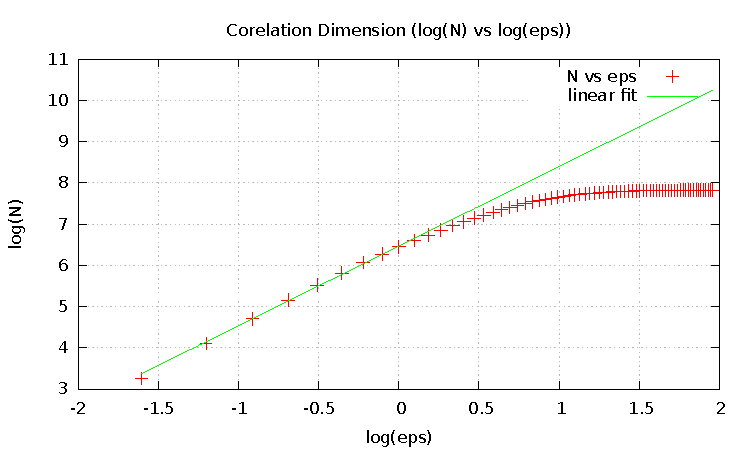
\includegraphics[width=12cm]{/home/atul/Documents/gitHub/chaosTerm/lorenzVersion1.3/output/dimensionCorrelation}

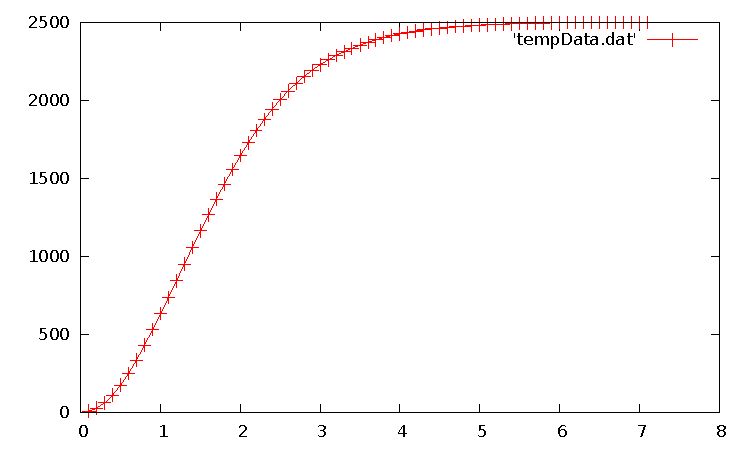
\includegraphics[width=12cm]{/home/atul/Documents/gitHub/chaosTerm/lorenzVersion1.3/output/dimension}

\lstset{     frame=single,     breaklines=true,     postbreak=\raisebox{0ex}[0ex][0ex]{\ensuremath{\color{red}\hookrightarrow\space}} }

\lstinputlisting{dimensionFit}


\section{Conclusion}

A lorenz attractor was simulated using RK4. Two lorenz attractors
were shown to get coupled, despite being in the chaotic regime. Interesting
periodic oscillations of the relative distance (measure of synchrony)
were found. These seem to naively said, contrad the theory. Two other
obvious ways of synchronization were attempted which seem to result
in a constant `phase difference' synchronization. This is indicated
by the relative distance seemingly varying slowly after the transience.
And finally, the correlation dimension of the lorenz attractor was
obtained to be very close to $\sim2$ as was expected.


\section{References and Acknowledgement}

I refered to the textbook for the course, titled \textbf{Nonlinear
Dynamics and Chaos}, \emph{S. H. Strogatz}, Perseus Books Publishing,
LCC

I would like to acknowledge our instructor, \emph{Prof. Sudeshna Sinha},
the instructor for the course by the same name.

I also mention the contribution of my friends (and colleagues). Foremost,
\emph{Vivek Sagar,} discussions with him accelerated the completion
of the work. In addition I thank \emph{Yosman Bapatdhar} and \emph{Arjit
Kant Gupta}, who were there when I wrote the first instance of the
code.


\section{Source Code}

The source code is available online at \url{https://github.com/toAtulArora/chaosTerm.git}.
The gnuplot\_fortran library has been mostly written by me (built
on top of a tutorial). Here I have appended only the main code.

\lstinputlisting[language=fortran]{lorenz2.f95}
\end{document}
